% !TEX program = pdflatex
% Compile from this directory with:
%   latexmk -pdf -interaction=nonstopmode -halt-on-error icsc.tex

\documentclass[runningheads]{llncs}

\usepackage[T1]{fontenc}
\usepackage{graphicx}
\usepackage{subcaption}
\usepackage{booktabs}
\usepackage{amsmath}
\usepackage{url}

\graphicspath{{figures/}}

\title{When the Same Insult Targets a Woman or a Man:\\
Human and LLM Perception of Gendered Attacks in Chinese}
\titlerunning{Human and LLM Perception of Gendered Attacks}

\author{Xuan Bao\inst{1} \and
Yiying Song\inst{1}\thanks{Corresponding author.} \and
Yueqin Hu\inst{1}\thanks{Corresponding author.}}
\authorrunning{X. Bao et al.}
\institute{Beijing Normal University, Beijing, China\\
\email{bxx520psycho@163.com}\\
\email{\{songyiying,yueqinhu\}@bnu.edu.cn}}

\begin{document}
\maketitle

\begin{abstract}
\textbf{Objective.} Large language models (LLMs) are increasingly used to rate hostile content, but whether they perceive Chinese gendered attacks the way human raters do remains unclear. We ask where human and LLM perceived attack ratings of Chinese gendered attacks are similar and where they differ when the target gender is the only thing that changes. \textbf{Method.} We constructed 371 Chinese gender-reversal minimal pairs of attack-laden sentences and collected ratings from nine contemporary LLMs and 779 valid Chinese participant sessions under three response formats (3-point category, 7-point Likert, 0--100 slider). The primary outcome was the paired female-minus-male attack-rating gap, $\Delta_{F-M}$, summarized by Cohen's $d_z$ and compared at four levels: direction, aggregate magnitude, domain profile across 10 attack categories, and item-level ordering. \textbf{Results.} Humans and LLMs agreed in direction (all 36 rater-by-scale cells had positive $\Delta_{F-M}$) and located the largest gender-differential effects in attacks on sexualization and appearance. They diverged in magnitude and item-level ordering: on the 3-point scale most LLMs sat between the male- and pooled-human references, while finer scales amplified LLM $d_z$ but dampened human $d_z$; item-level $\mathrm{ICC}(2,1)$ remained below 0.25 even when aggregate $d_z$ values nearly coincided. \textbf{Conclusion.} Humans and LLMs share the direction and broad content structure of perceived gendered attack ratings in Chinese, but agreement is conditional on the human reference group, the response scale, and the analytic level; LLM judgements of subjective social content should therefore be reported as a structured profile, not as a single global agreement score.

\keywords{Large language models \and Gendered attacks \and Hate speech \and Minimal pairs \and Social computing.}
\end{abstract}

\section{Introduction}

Online hate and harassment undermine individual well-being, public discourse, and platform governance \cite{schoenebeck2023}. In Chinese-language online spaces, gender has become one of the most visible axes of such hostility: studies of major Chinese platforms document sexist and misogynistic language, the stigmatization of feminism, and platform dynamics that amplify gender antagonism \cite{jiang2021,jingschmidt2018,liao2024}. Yet a basic question about how this hostility is \emph{perceived} remains open. When the same hostile sentence is directed at a woman rather than a man, with only the gender of the target changed and the attack content held fixed, do raters perceive it as more attacking? And when both humans and large language models (LLMs) are asked to rate such sentences, do they agree on \emph{whether}, \emph{how much}, and \emph{where} the gender-targeted version is more attacking?

This question is socially consequential and methodologically tractable at the same time. Whether the same content is perceived as more attacking when directed at a woman is itself a documented effect in early experimental work on hate-speech judgements that manipulated the target group \cite{cowan1996}, and recent large-scale comparisons of human and LLM annotators show that perceived severity varies systematically with the target's social attributes \cite{giorgi2025}. Hate-speech annotation labels also vary with annotator demographics rather than being a neutral gold standard \cite{sap2019,larimore2021,davani2022,santy2023}, and existing benchmark datasets entangle target identity with content extremity and topic \cite{mathew2021}, so the question of who perceives what is part of the data, not external to it. Controlled contrastive testing, including minimal-pair manipulations, has emerged as a way to isolate a single input feature from confounding content \cite{ribeiro2020,rottger2021}.

LLMs are now used routinely to annotate, score, and moderate hostile text in places where human coders were previously the only option \cite{he2024,ziems2024,chiu2022,davidson2026}, and these LLM judgements do not simply reproduce human socio-demographic variation \cite{sun2025,orlikowski2025}. For Chinese gendered attacks, however, no controlled comparison has yet asked the basic perceptual question above. We close this gap with 371 Chinese gender-reversal minimal pairs of attack-laden sentences: within each pair, the female-targeted and male-targeted versions contain the same attack content and differ only in the gender referent. Ratings were collected from nine contemporary LLMs and 779 valid Chinese participant sessions under three response formats (a 3-point category scale, a 7-point Likert scale, and a 0--100 slider). The primary outcome is the paired female-minus-male perceived attack-rating gap, $\Delta_{F-M}$, summarized by Cohen's $d_z$ across the 371 items.

Comparing humans and LLMs on this design requires more than a single agreement number. We separate four levels at which agreement can hold or break: the \emph{direction} of the effect (do both place female-targeted versions on the same side of zero?), the \emph{aggregate magnitude} (do they agree on how big the gap is?), the \emph{domain profile} (do the largest gaps occur in the same attack domains?), and the \emph{item-level ordering} (do the same individual sentences carry the effect?). The same comparison is conducted against three human reference groups (pooled human aggregate, female participants, male participants) and across the three response formats, because subjective ratings depend on both the response interface \cite{lozano2008,preston2000} and the rater group, and these dependencies are part of what we measure rather than nuisance to be averaged over. Throughout, we use \emph{alignment} in this behavioural sense: similarity between human and LLM ratings on the same items, not RLHF or value alignment in the safety-tuning sense.

The story that emerges is one of striking similarity in some places and equally striking divergence in others. Humans and LLMs agree that female-targeted versions of the same insult are perceived as more attacking on average, and both locate the largest gender-differential effects in attacks on \emph{sexualization} and \emph{appearance}. But the size of the gap differs from the human reference group one compares against, the gap behaves in opposite directions across humans and LLMs as the rating scale becomes finer, and item-level correspondence is weak even when aggregate effects are close. The rest of the paper presents this pattern, and the Discussion returns to what it means for using LLMs as raters of subjective social content.

\section{Design and Measures}

\subsection{Materials}

A native Chinese-speaking research team constructed 371 minimal pairs of attack-laden sentences, yielding 742 gender-targeted sentence versions. The item pool was built from a three-level coding framework derived from prior work on gendered derogation, inductive review of hostile expressions in Chinese social-media contexts, and iterative team coding. The framework was designed to cover common forms of interpersonal attack and comprised 10 first-level attack domains, 71 second-level categories, and more than 180 third-level categories. The main analyses use only the first level: sexualization, appearance, gender role or expression, interpersonal relations, moral character, economic resources, social status, emotional stability, capability or competence, and intellectual rationality.

The coding framework was developed by integrating prior literature on interpersonal derogation, gendered hostility, online sexism, and person evaluation with inductive coding of attack expressions on major Chinese social-media and forum platforms (Weibo, Tieba, Xiaohongshu, Douban, and Hupu). Sentence templates were drafted from naturally occurring online language and AI-assisted writing, with all candidates manually reviewed by the research team; items that sounded unnatural, depended on platform-specific context, or could not be reversed without changing the attack content were rewritten or removed, reducing an initial pool of approximately 400 candidates to 371 templates. Three native Chinese-speaking coders with psychology training then reviewed every item for naturalness, attack presence, domain fit, and minimal-pair equivalence, with disagreements resolved through discussion. Within each pair, the two versions are identical except for a gender-referent substitution (e.g., female versus male pronouns, gendered nouns, names, or kin terms), which lets us attribute residual paired rating gaps to the gender manipulation rather than to selection on content extremity, a confound endemic to natural-language gender comparisons (Fig.~\ref{fig:natural-confound}).

\begin{figure}[t]
  \centering
  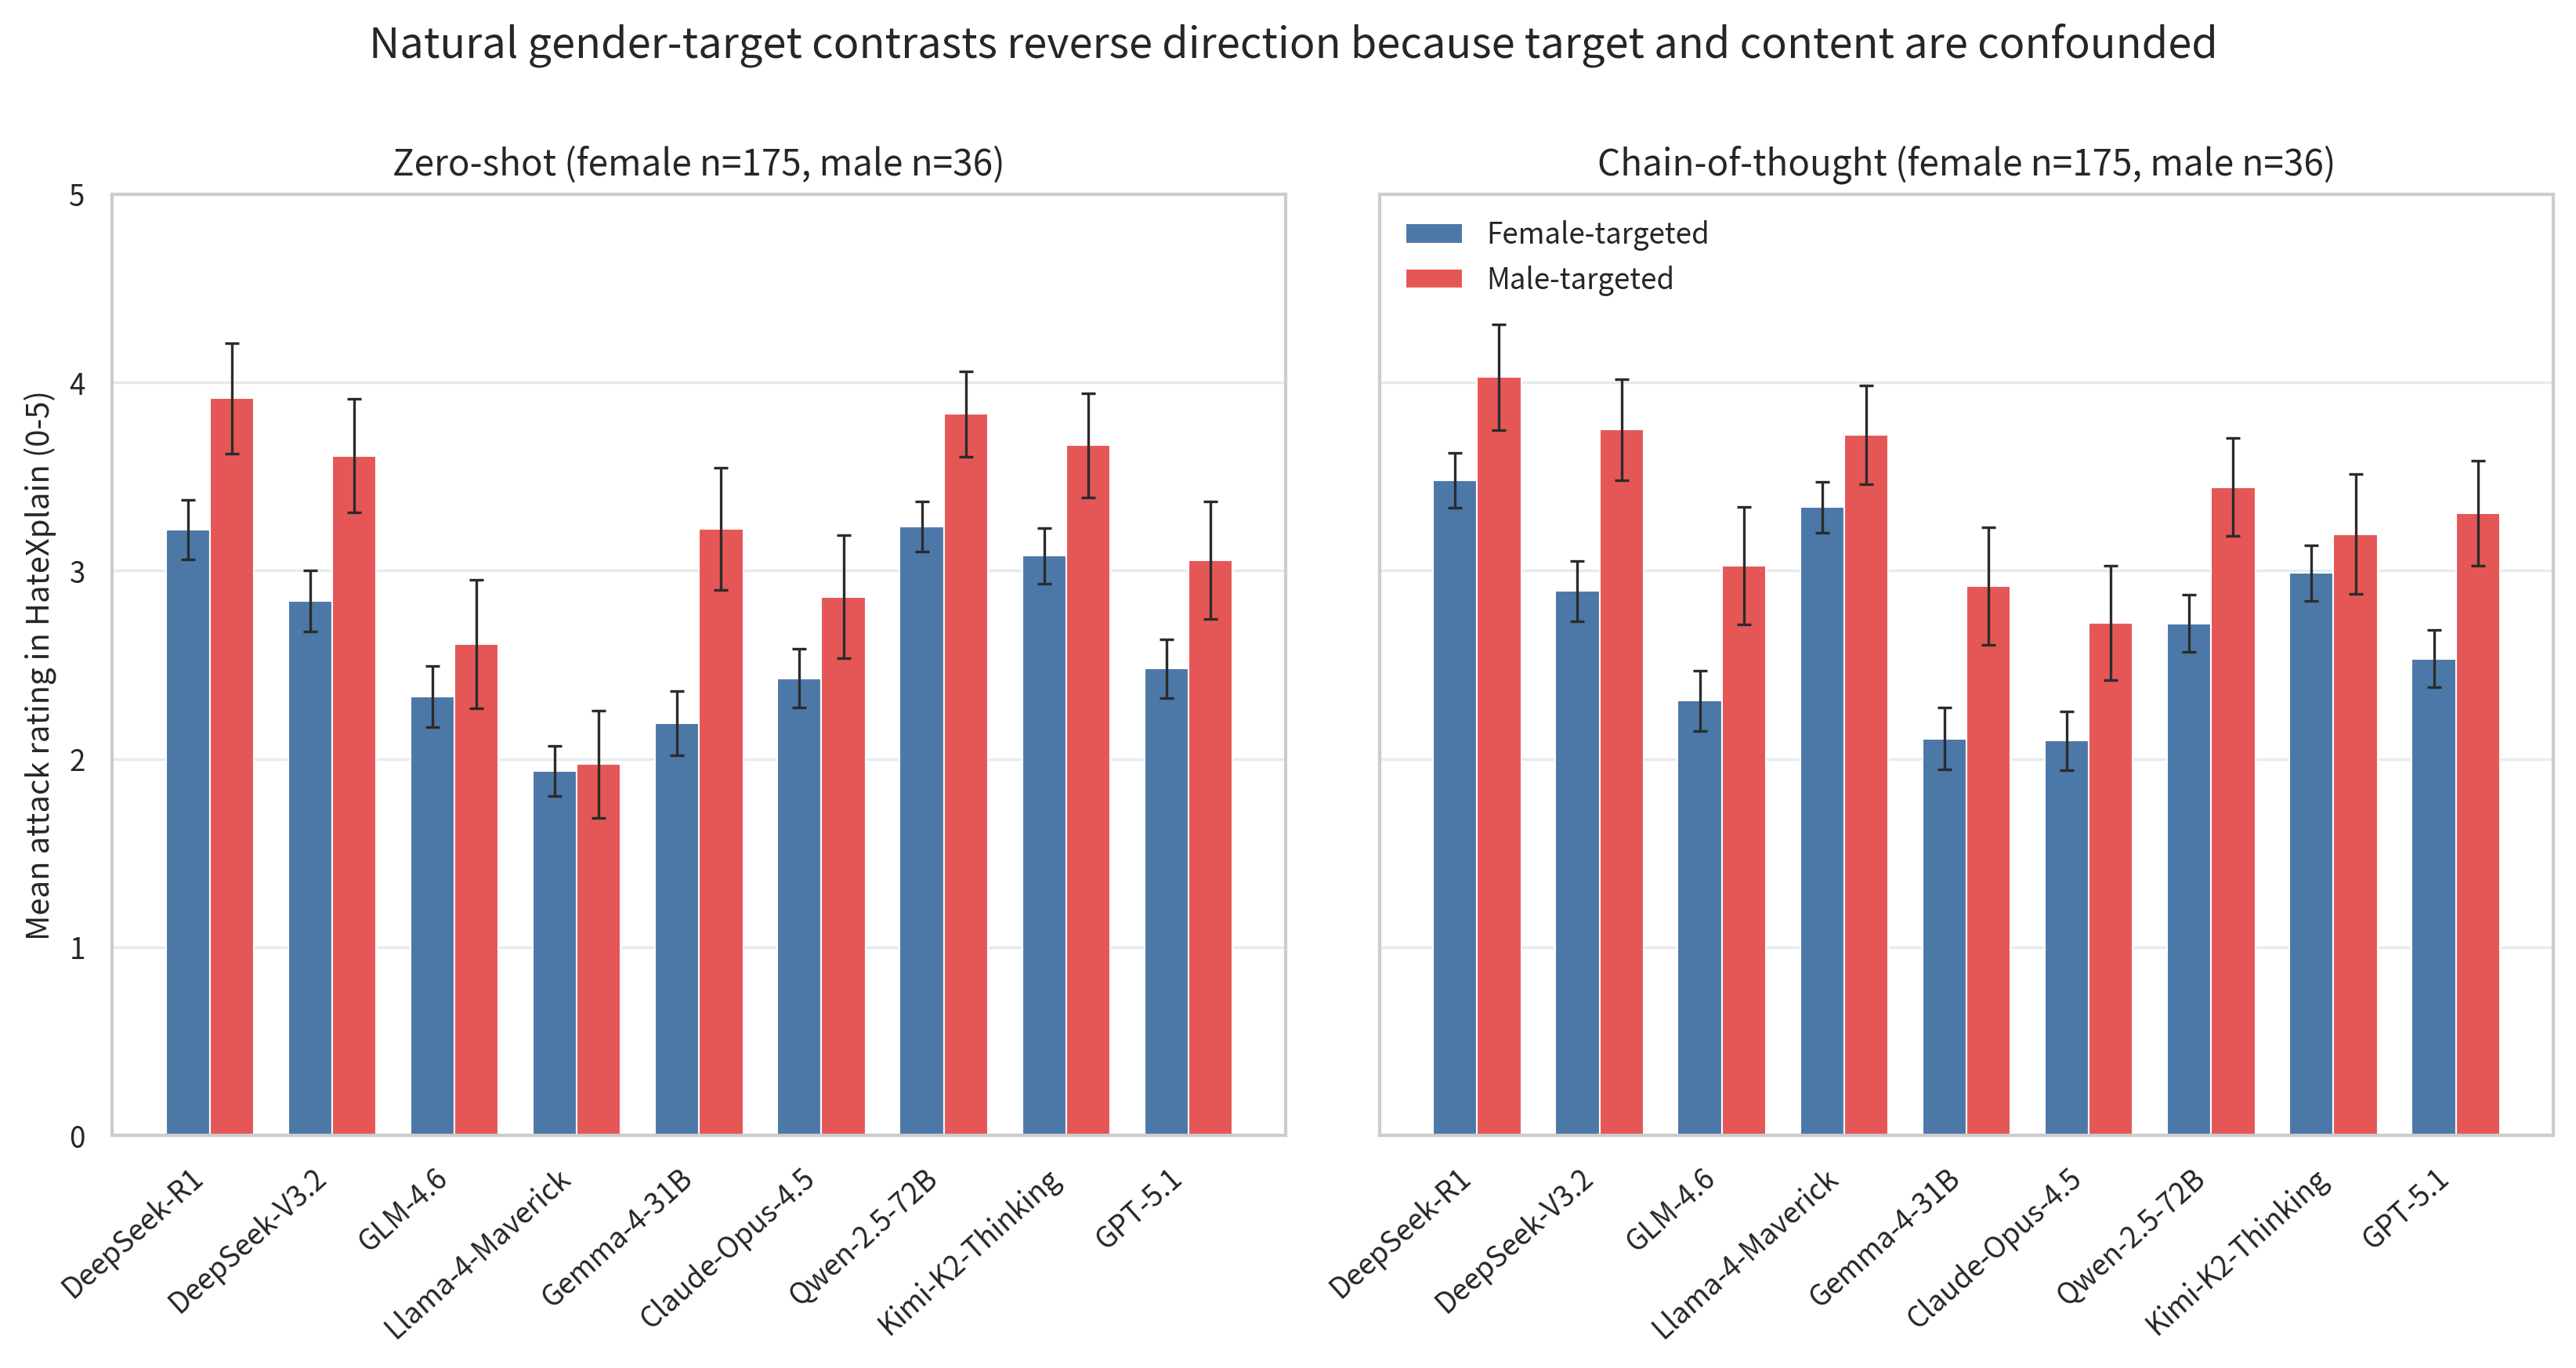
\includegraphics[width=\linewidth]{fig_r1_natural_gender_target_confound.pdf}
  \caption{Why a controlled minimal-pair design is necessary. In an English HateXplain subset stratified by target gender, female-targeted posts are more numerous but male-targeted posts receive higher mean LLM perceived attack ratings, because target gender co-occurs with content extremity and topic. Raw female-versus-male contrasts in naturally occurring corpora therefore cannot identify the target-gender effect.}
  \label{fig:natural-confound}
\end{figure}

\subsection{Raters and Response Formats}

Nine production LLMs were queried in November 2025: Claude-Opus-4.5, DeepSeek-R1, DeepSeek-V3.2, Gemma-4-31B, Llama-4-Maverick, Kimi-K2-Thinking, GPT-5.1, Qwen-2.5-72B-Instruct, and GLM-4.6. Each model rated both versions of every pair under each response format.

The human sample contained 779 valid Chinese rating sessions from 712 unique participants. Participants were randomly assigned to one response format and rated a pseudo-random subset of about 75 sentence versions. The design avoided showing both versions of the same minimal pair to the same participant. Human item means were therefore estimated across participants and then paired at the template level. Because later analyses compare female- and male-participant references, Table~\ref{tab:human-balance} reports the participant-gender balance within each response format.

\begin{table}[t]
  \centering
  \small
  \caption{Valid human rating sessions by participant gender and assigned response format.}
  \label{tab:human-balance}
  \begin{tabular}{lrrr}
    \toprule
    Response format & Female participants & Male participants & Total \\
    \midrule
    3-point category & 134 & 134 & 268 \\
    7-point Likert & 128 & 116 & 244 \\
    0--100 slider & 130 & 137 & 267 \\
    \midrule
    Total & 392 & 387 & 779 \\
    \bottomrule
  \end{tabular}
\end{table}

The three formats were: a 3-point category scale (0 = not attacking, 1 = mildly attacking, 2 = strongly attacking), a 7-point scale from 0 to 6, and a 0--100 slider. These formats represent coarse annotation, conventional graded judgement, and high-granularity perceived intensity.

\subsection{Estimand}

For item $i$, rater group $r$, and scale $c$, the paired target-gender gap is
\[
  \Delta^{(i)}_{F-M}(r,c)=s^{(i)}_F(r,c)-s^{(i)}_M(r,c),
\]
where $s_F$ and $s_M$ are the female- and male-targeted item means. The summary effect size is Cohen's paired $d_z$,
\[
  d_z(r,c)=
  \frac{\overline{\Delta^{(i)}_{F-M}(r,c)}_i}
  {\widehat{\mathrm{SD}}\left(\Delta^{(i)}_{F-M}(r,c)\right)_i},
\]
computed over the 371 item pairs. This makes items, rather than individual ratings, the common unit for human and LLM comparisons.

\section{Results}

\subsection{Direction: humans and LLMs both rate female-targeted versions as more attacking}
\label{sec:r-direction}

All 36 rater-by-scale cells produced a positive mean $\Delta_{F-M}$: the female-targeted version received a higher mean rating than the male-targeted version (Fig.~\ref{fig:direction}). Among human raters, female-targeted versions received higher aggregated item ratings for 58.2\%--74.7\% of items, depending on participant group and scale. Among LLMs, 3-point-scale ratings frequently produced identical values for the female- and male-targeted versions of the same item pair; all 27 model-by-scale cells nevertheless produced a positive mean $\Delta_{F-M}$, with BH-FDR adjusted $q<10^{-7}$ for $\Delta_{F-M}>0$.

\begin{figure}[t]
  \centering
  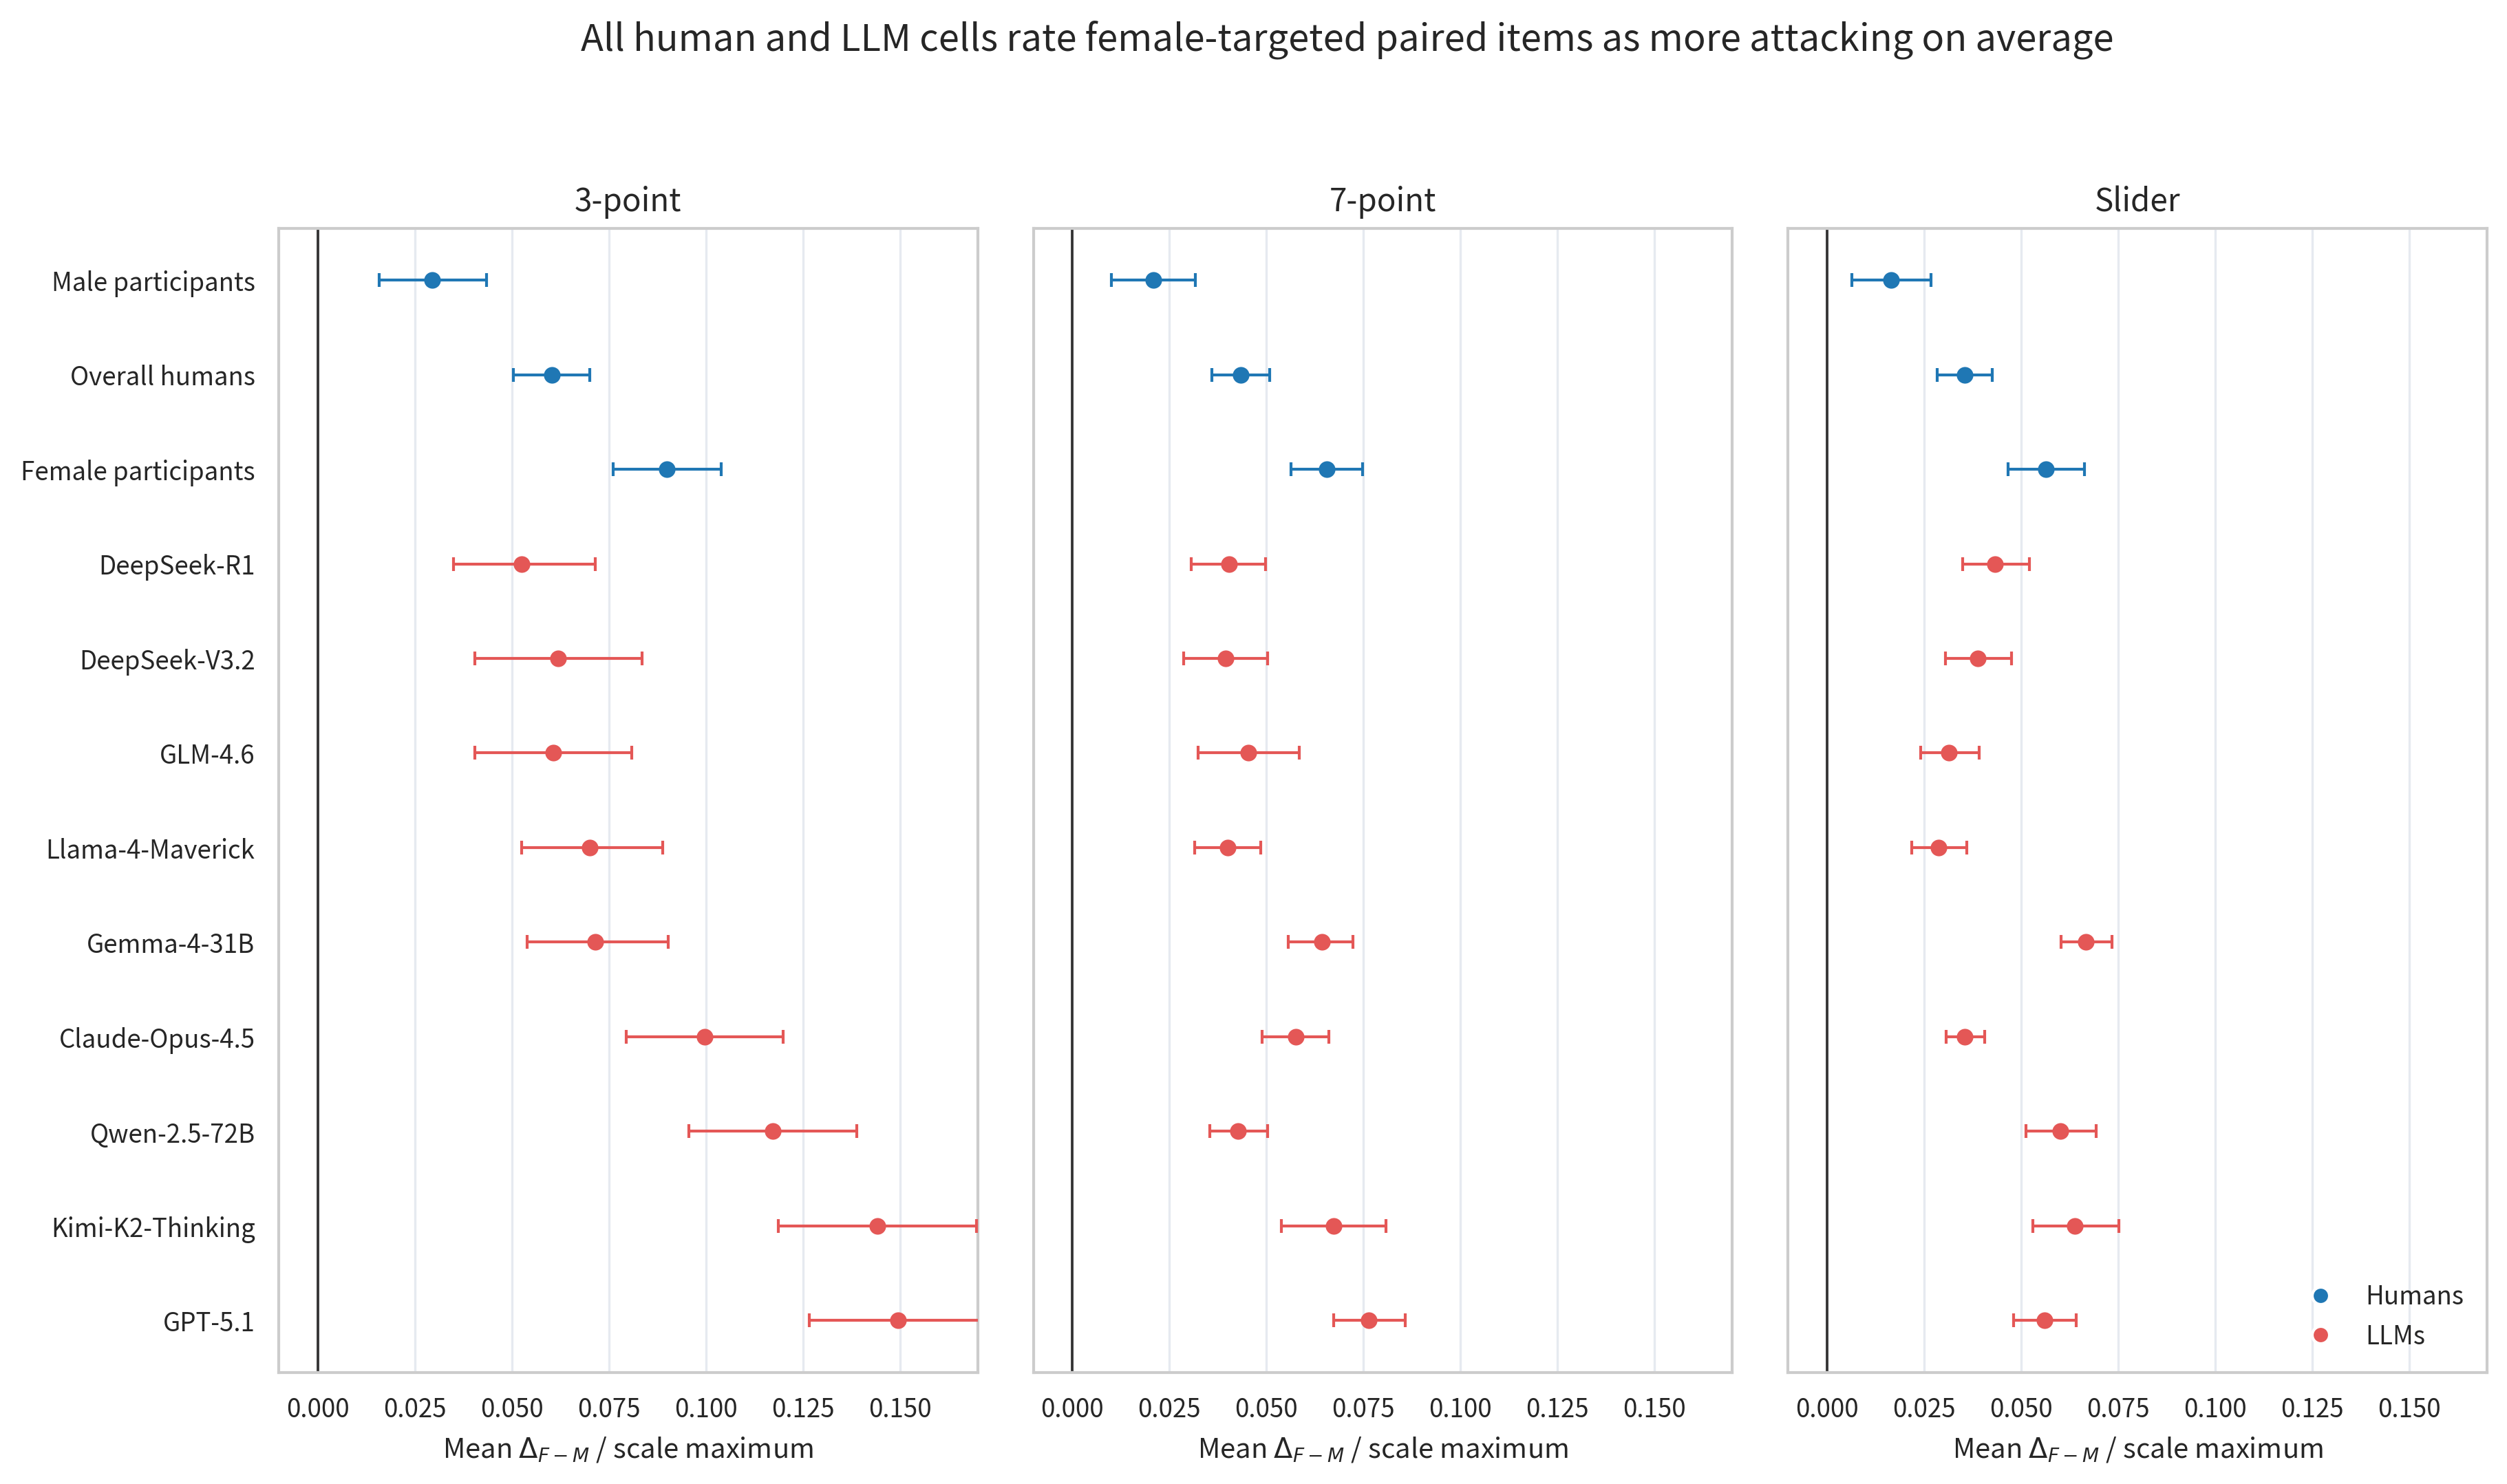
\includegraphics[width=\linewidth]{fig_r2_direction_agreement_forest.pdf}
  \caption{Direction-level agreement across human and LLM raters. Points show normalized mean paired female-minus-male rating gaps; intervals are item-level bootstrap 95\% intervals over the 371 pairs.}
  \label{fig:direction}
\end{figure}

Humans and LLMs therefore agree on the direction of the target-gender effect; the next sections examine whether they also agree on its magnitude, on its location across attack domains, and on its placement at the item level.

\subsection{Magnitude: human--LLM gaps depend on the reference group and on the rating scale}
\label{sec:r-magnitude}

\textbf{On the 3-point scale.} Among our three formats, the 3-point scale is the most categorical and closest in granularity to the small label sets commonly used in hate-speech annotation, such as the three-label schemes of HateXplain \cite{mathew2021} and SWSR \cite{jiang2021}; we therefore anchor the magnitude comparison here. The human reference values were $d_z=0.219$ for male participants, $d_z=0.621$ for the pooled human aggregate, and $d_z=0.655$ for female participants. The nine LLMs ranged from $d_z=0.289$ to $0.653$ (Table~\ref{tab:threepoint}): all nine exceeded the male-participant $d_z$, eight fell in the segment $[d_z^{\text{male}}, d_z^{\text{pooled}})$, one (GPT-5.1, $d_z=0.653$) fell in $[d_z^{\text{pooled}}, d_z^{\text{female}})$, and none reached or exceeded the female-participant $d_z$ (Fig.~\ref{fig:reference}).

\begin{table}[t]
  \centering
  \small
  \caption{3-point summary. Means are normalized by scale maximum and rows are sorted within blocks by $d_z$.}
  \label{tab:threepoint}
  \begin{tabular}{lccc}
    \toprule
    Rater & Mean M & Mean F & $d_z$ \\
    \midrule
    Male participants & 0.573 & 0.602 & 0.219 \\
    Overall humans & 0.562 & 0.622 & 0.621 \\
    Female participants & 0.552 & 0.642 & 0.655 \\
    \midrule
    DeepSeek-R1 & 0.892 & 0.945 & 0.289 \\
    DeepSeek-V3.2 & 0.807 & 0.869 & 0.289 \\
    GLM-4.6 & 0.846 & 0.907 & 0.297 \\
    Llama-4-Maverick & 0.784 & 0.854 & 0.379 \\
    Gemma-4-31B & 0.902 & 0.973 & 0.408 \\
    Claude-Opus-4.5 & 0.834 & 0.934 & 0.498 \\
    Qwen-2.5-72B & 0.796 & 0.914 & 0.553 \\
    Kimi-K2-Thinking & 0.709 & 0.853 & 0.572 \\
    GPT-5.1 & 0.737 & 0.887 & 0.653 \\
    \bottomrule
  \end{tabular}
\end{table}

\begin{figure}[t]
  \centering
  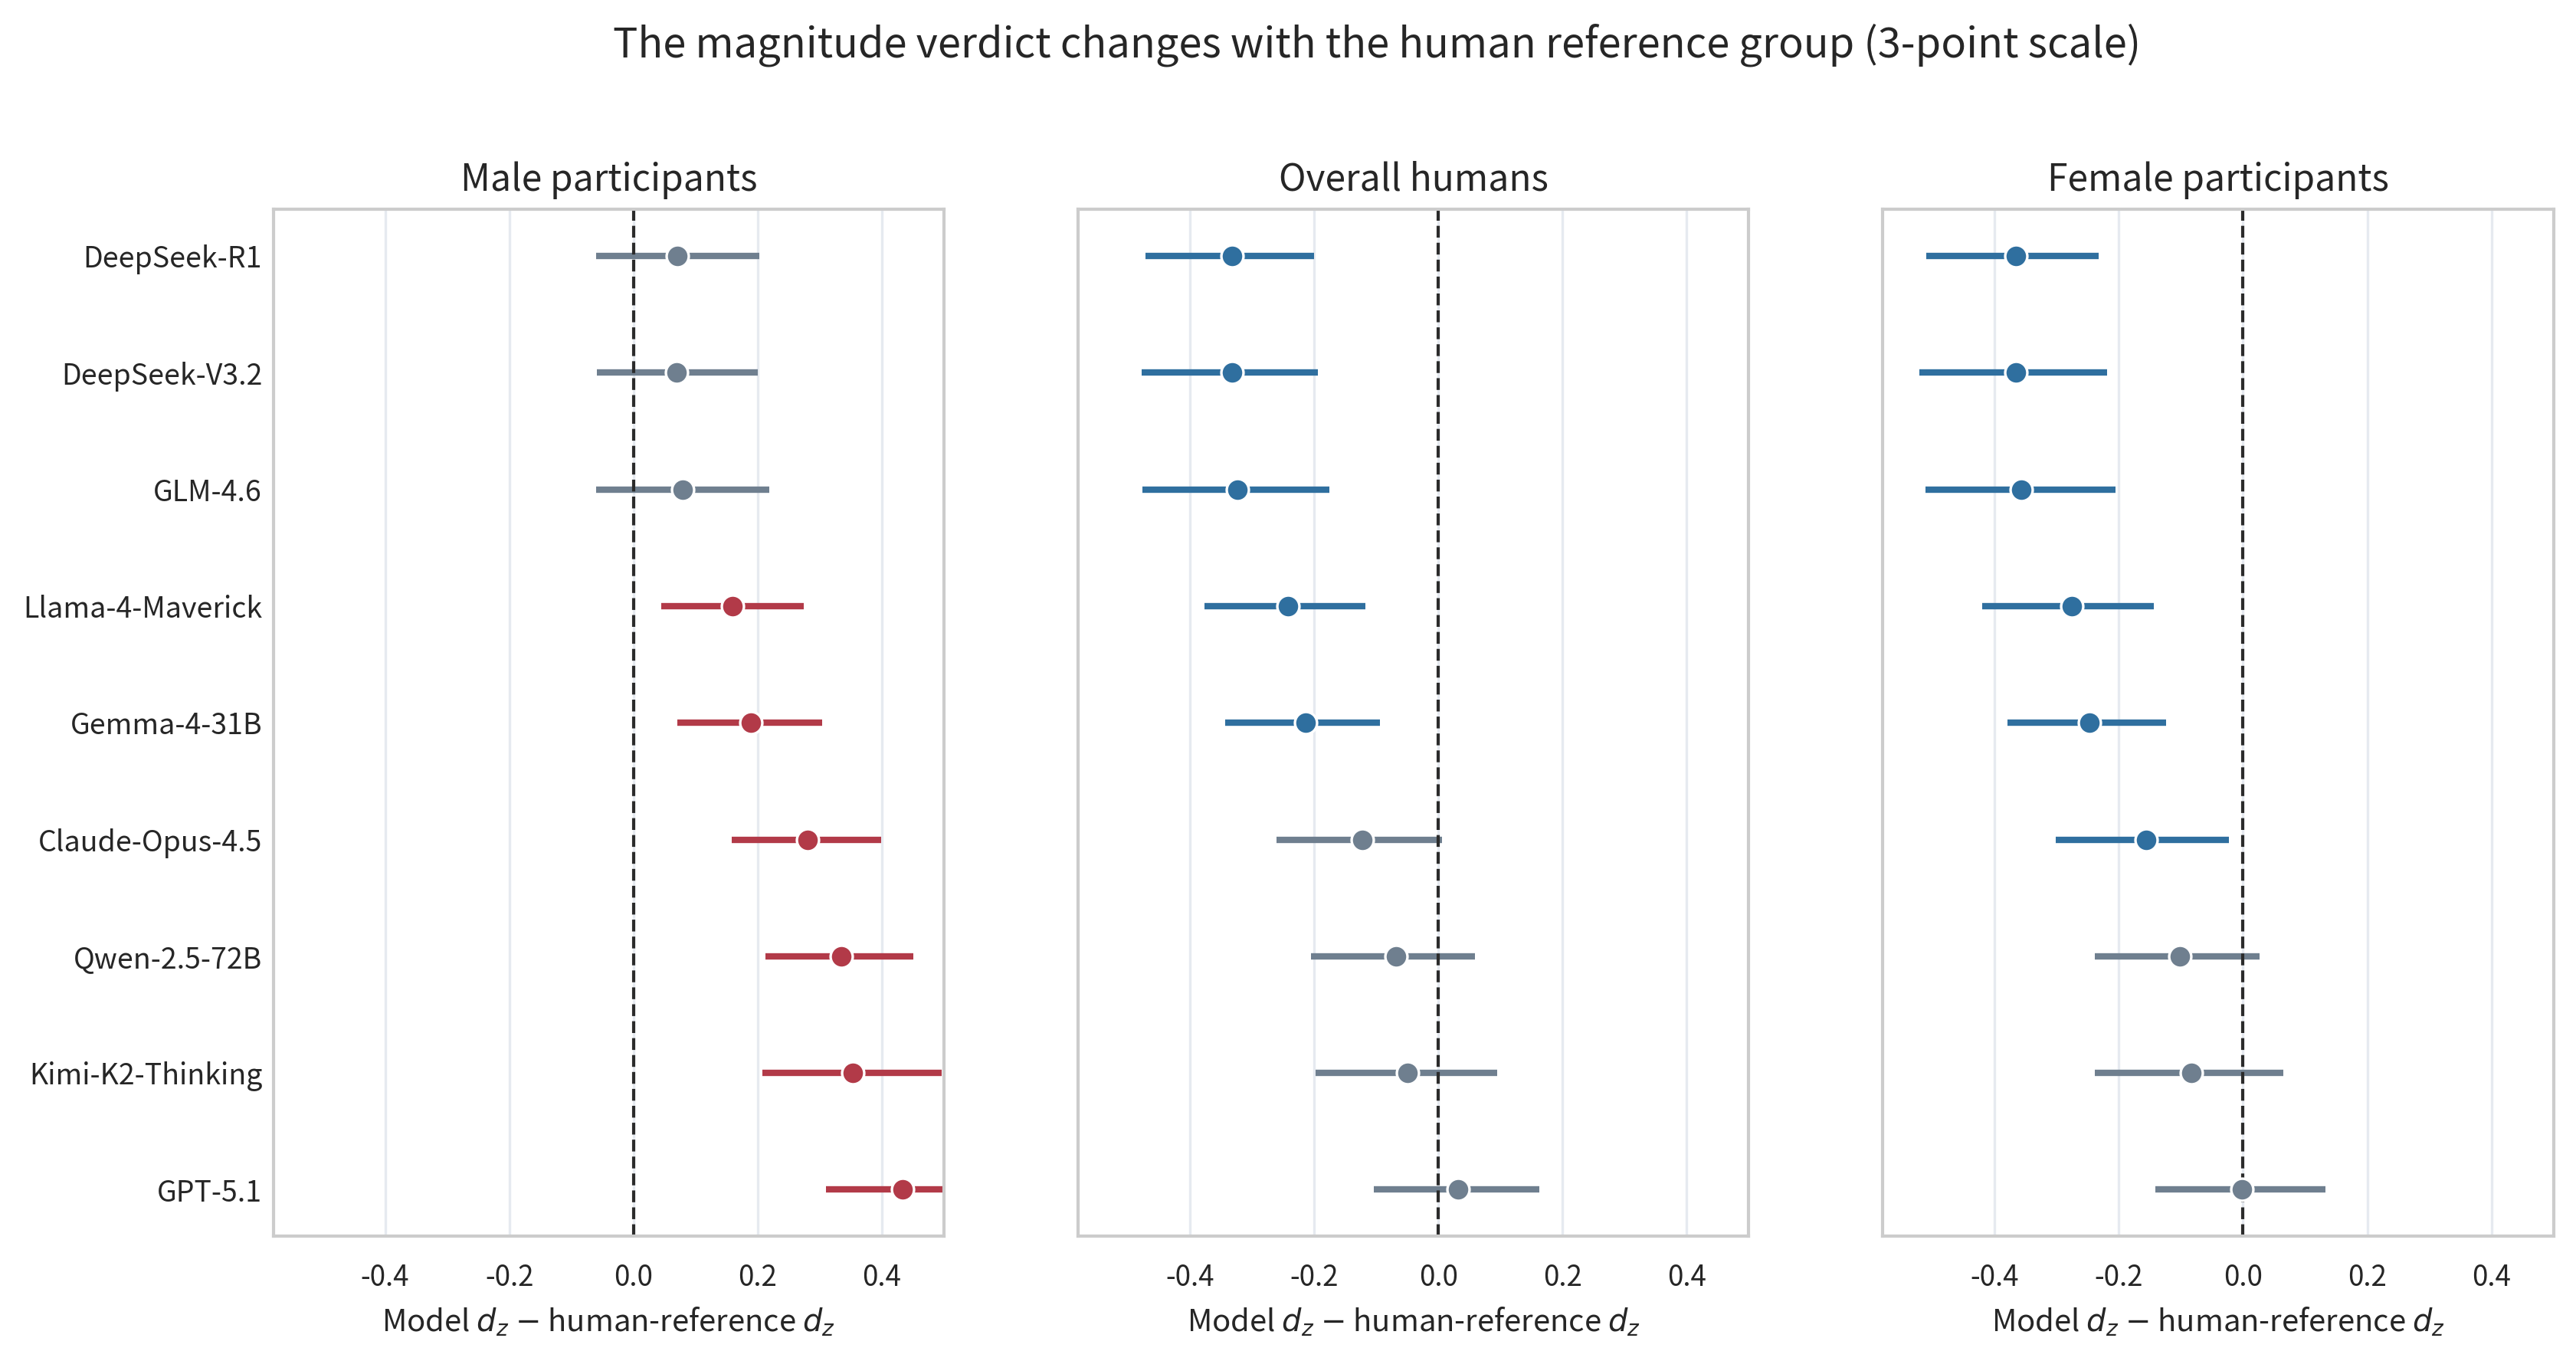
\includegraphics[width=\linewidth]{fig_r3_reference_group_delta_dz_forest.pdf}
  \caption{3-point magnitude comparison. Each point is an LLM's $d_z$ minus the human-reference $d_z$; intervals are item-level bootstrap 95\% intervals.}
  \label{fig:reference}
\end{figure}

\textbf{Across response formats.} As the response format became finer, human $d_z$ values stayed flat or declined while most LLM $d_z$ values rose. Overall humans moved from $d_z=0.621$ to $0.588$ to $0.512$, male participants from $0.219$ to $0.198$ to $0.167$, and female participants from $0.655$ to $0.704$ to $0.590$. Six of the nine LLMs showed monotonic or near-monotonic increases over the same sequence, with Gemma-4-31B rising from $0.408$ to $0.773$ to $1.016$; the remaining three were flatter or non-monotonic (Fig.~\ref{fig:scale}). The LLM panel therefore shifted upward relative to the human references as the rating scale became finer: the number of LLMs at or above the pooled-human $d_z$ was one of nine on the 3-point scale, three of nine on the 7-point scale, and five of nine on the slider; the corresponding counts at or above the female-participant $d_z$ were zero, two, and five.

\begin{figure}[t]
  \centering
  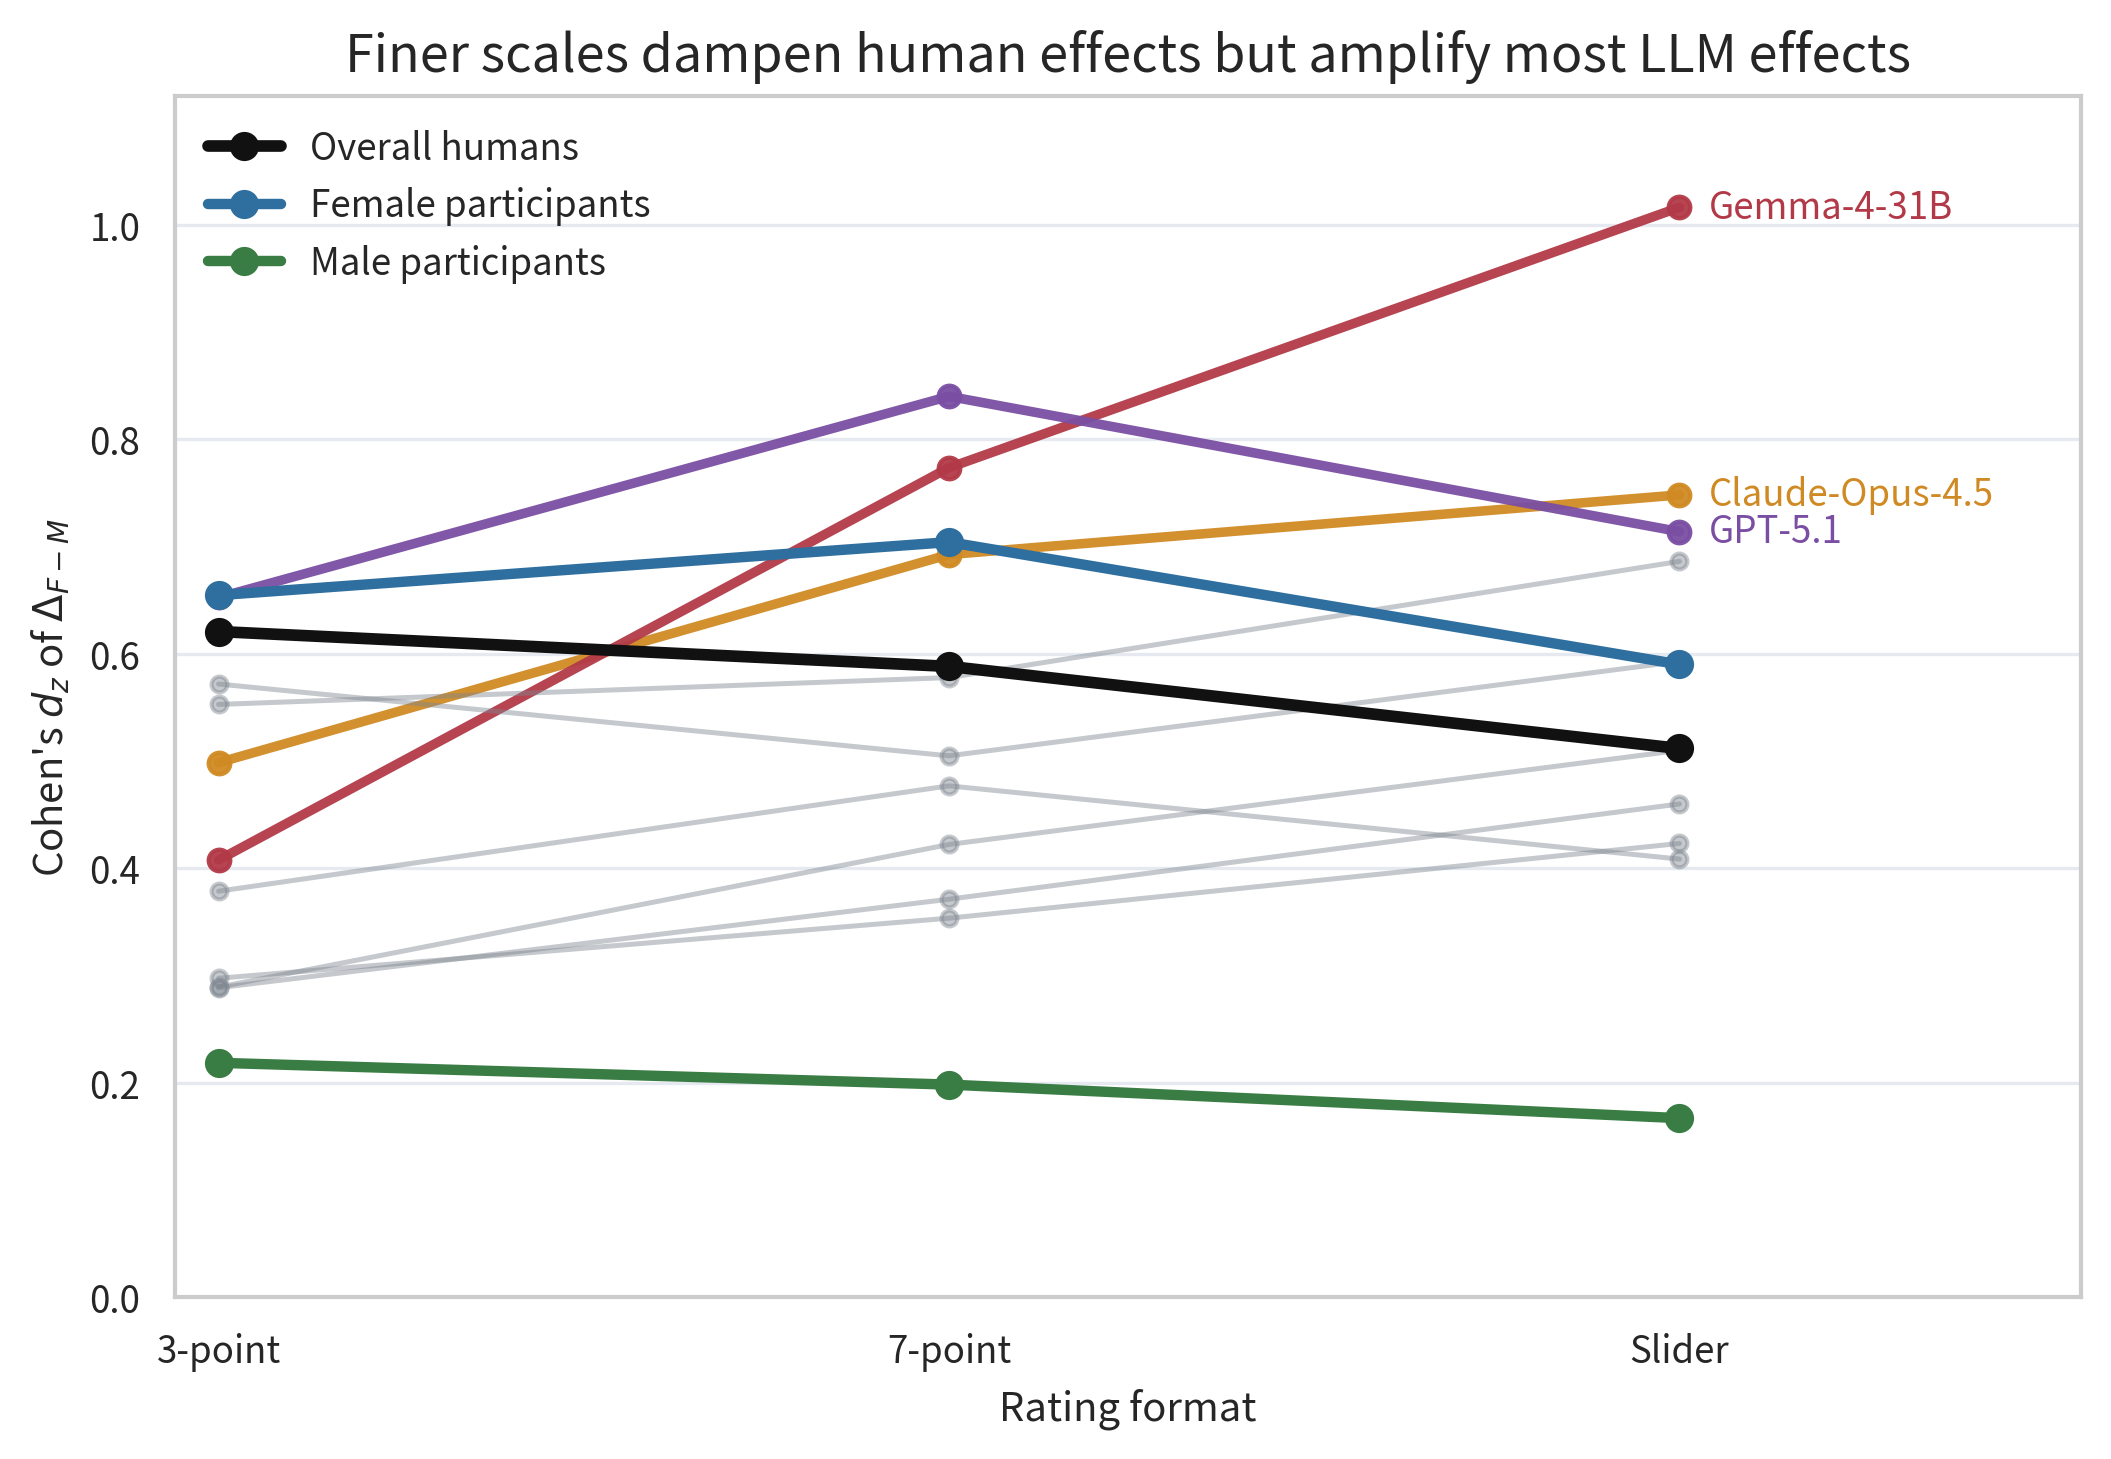
\includegraphics[width=.82\linewidth]{fig_r5_scale_response_trajectory.pdf}
  \caption{Cohen's $d_z$ across 3-point, 7-point, and slider formats for each human stratum and each LLM. Human curves stay flat or decline; most LLM curves rise.}
  \label{fig:scale}
\end{figure}

\subsection{Domain profile: both humans and LLMs locate the largest gender effects in sexualization and appearance}
\label{sec:r-domain}

For overall humans, sexualization had $d_z=1.47$, $1.42$, and $1.18$ across the 3-point, 7-point, and slider formats; appearance had $d_z=0.76$, $0.80$, and $0.61$. Sexualization and appearance were the two largest-$d_z$ domains for overall humans, for female participants, and for the LLM median across all three formats; for male participants the same two domains carried their largest positive values, with smaller magnitudes overall (Fig.~\ref{fig:domain}).

\begin{figure}[t]
  \centering
  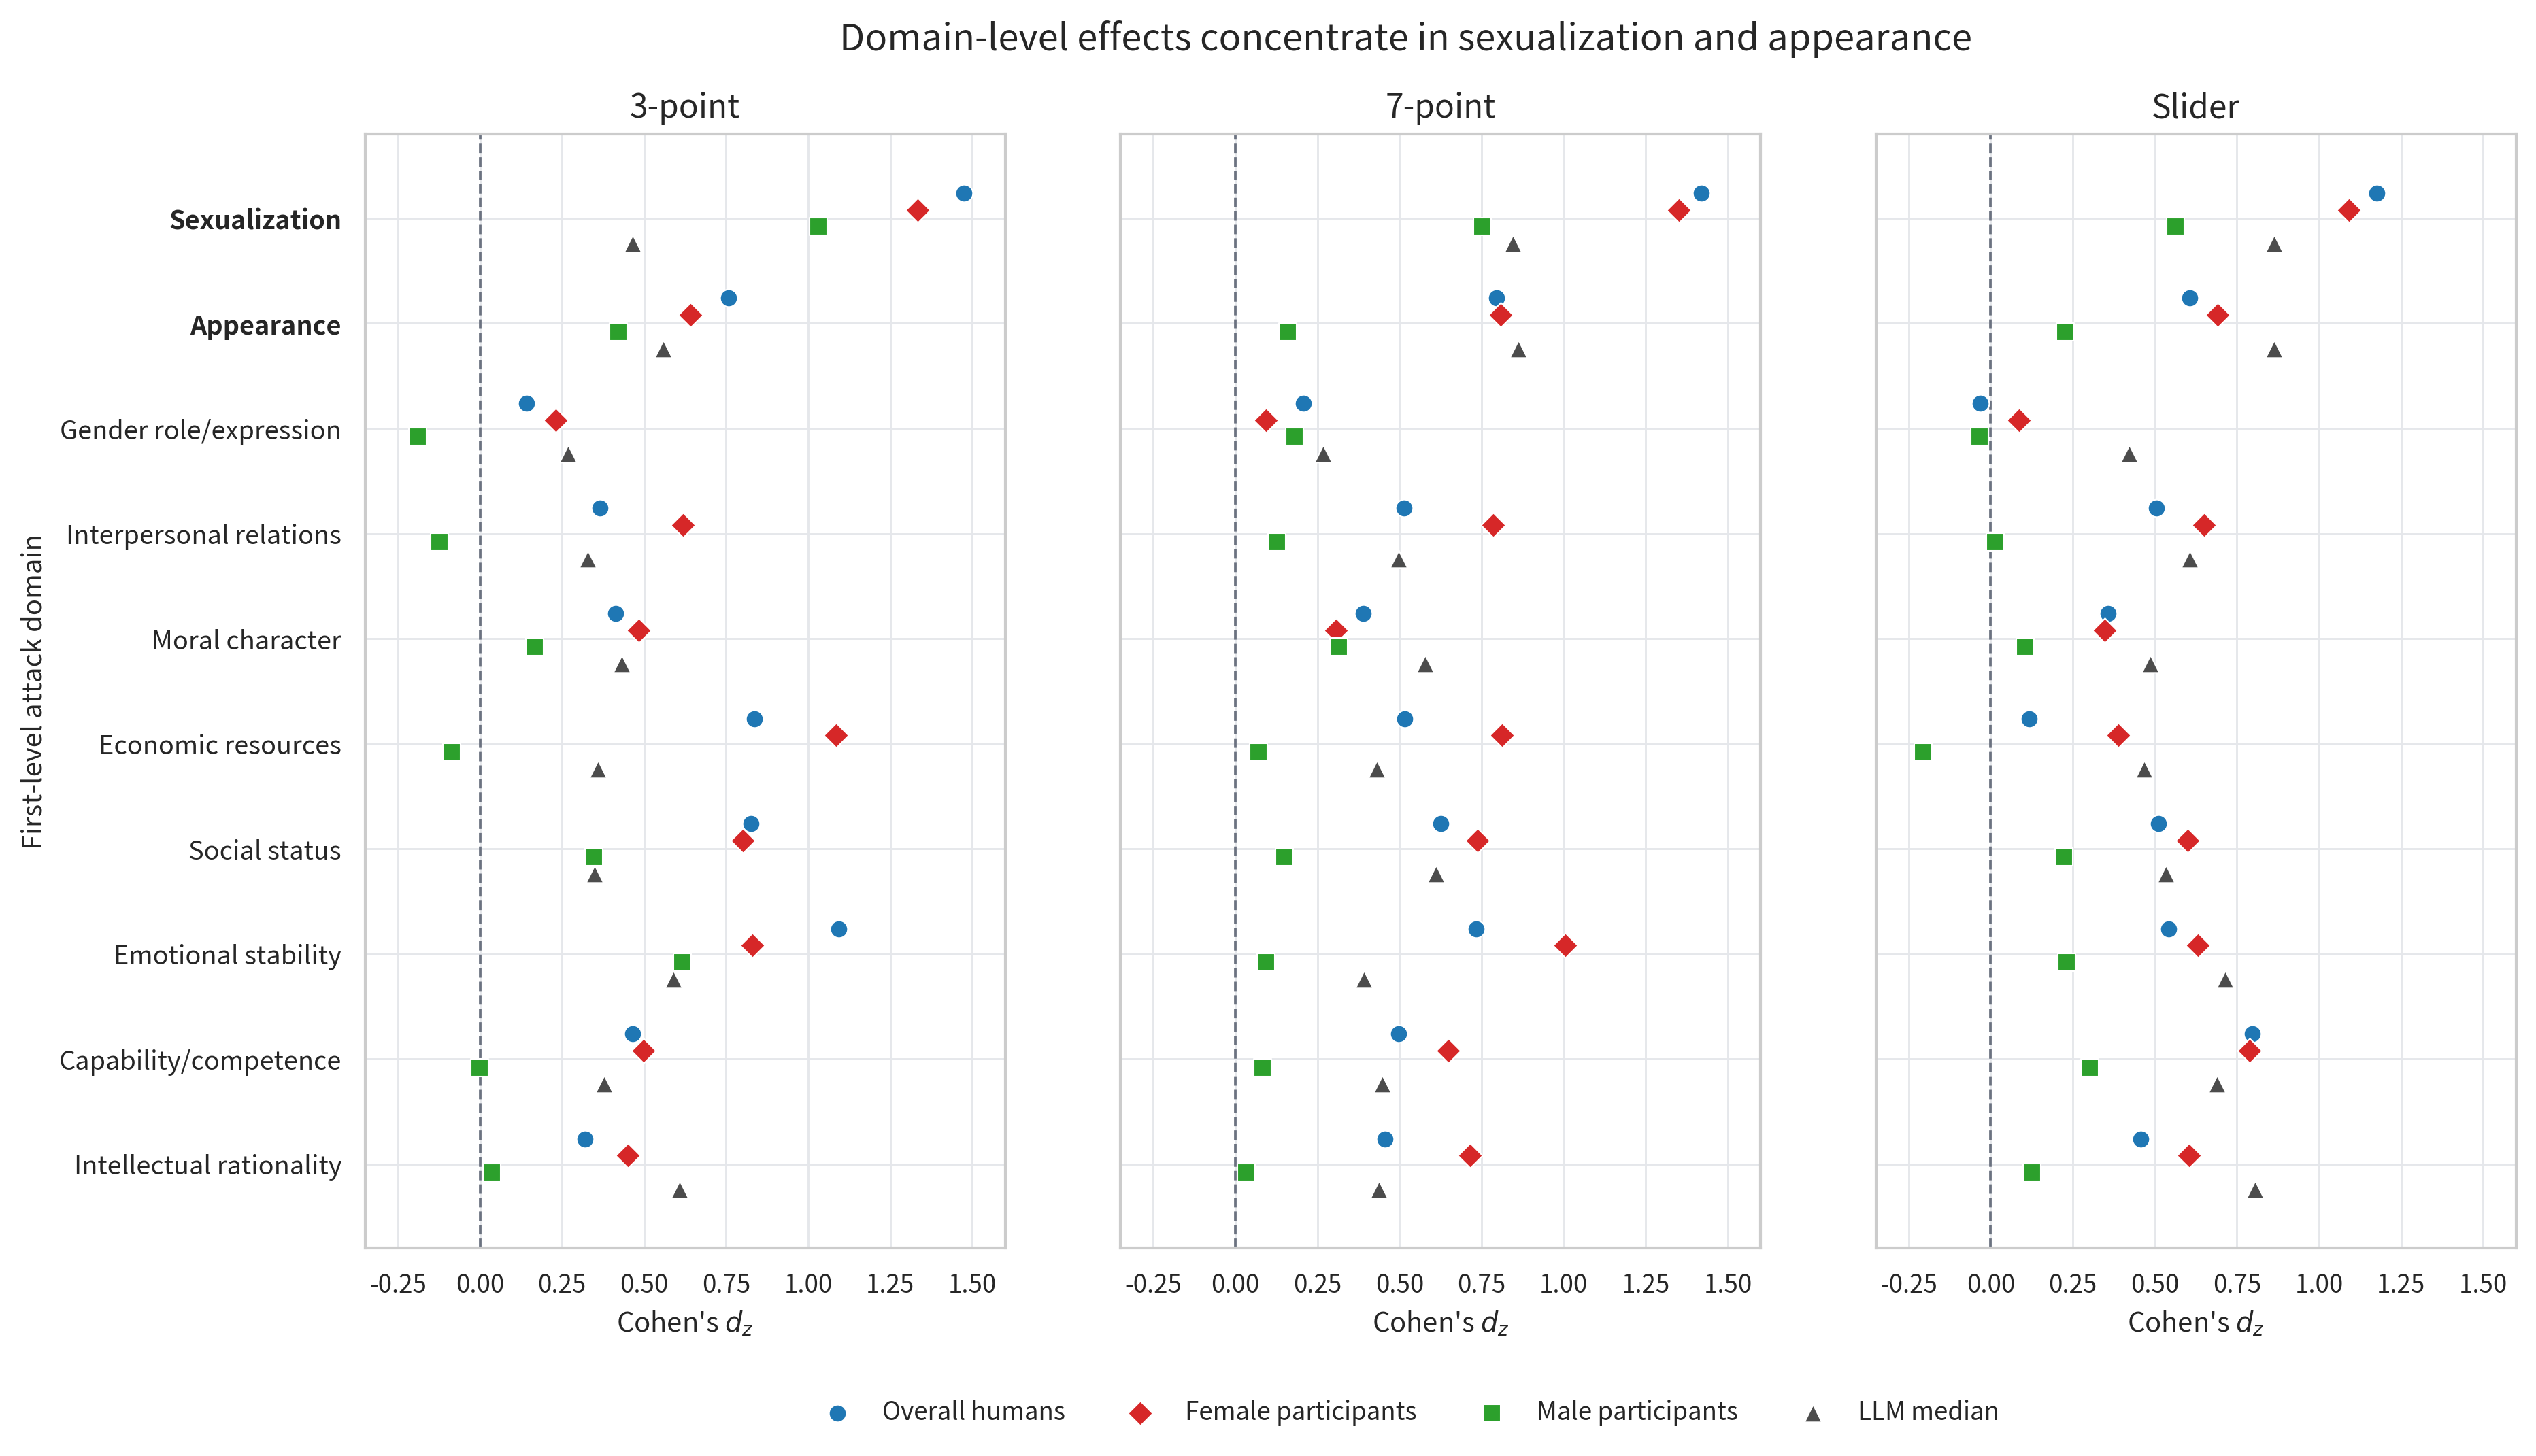
\includegraphics[width=\linewidth]{fig_r4_domain_alignment_forest.pdf}
  \caption{Domain-profile view of Cohen's $d_z$ for the female-minus-male gap across response formats. Points show the three human strata and the LLM median; sexualization and appearance are consistently the two largest-$d_z$ domains.}
  \label{fig:domain}
\end{figure}

The Spearman correlations between human and LLM $d_z$ vectors across the 10 domains (Table~\ref{tab:levels}) ranged from $0.56$ to $0.85$ for the best model in each cell. With only 10 domains, the chance baseline is wide: under a permutation null over 10 items, the two-sided $95\%$ Spearman interval is approximately $[-0.65, +0.65]$, so a $|\rho|$ value must exceed roughly $0.65$ to be distinguishable from random ranking at this granularity. Seven of the nine best-model cells exceeded this cutoff; two cells, both anchored on the female-participant reference (Gemma at $\rho=0.56$ on the 3-point scale and Gemma at $\rho=0.64$ on the 7-point scale), did not. On the 3-point scale, some LLMs ranked appearance above sexualization or compressed the gap between them; on the 7-point and slider formats the sexualization-above-appearance ordering was more consistently reproduced.

\subsection{Levels of agreement: no single LLM is closest to humans on every dimension}
\label{sec:r-levels}

We summarize the human--LLM agreement at three analytic levels: \emph{aggregate similarity} as $|d_z^{\text{LLM}}-d_z^{\text{human}}|$, \emph{domain-profile similarity} as the Spearman correlation between the human and LLM $d_z$ vectors across the 10 domains, and \emph{item-level similarity} as $\mathrm{ICC}(2,1)$ between the human and LLM $\Delta_{F-M}^{(i)}$ values across the 371 pairs. Table~\ref{tab:levels} lists the closest LLM for each level $\times$ human-reference $\times$ scale combination; within each row, the closest model is generally different across the three columns, and the closest model also varies across rows. The item-level ICC values ranged from $0.089$ to $0.222$ for the best model in each cell. Figure~\ref{fig:levels}(a) shows the same closest-model information visually, and Fig.~\ref{fig:levels}(b) shows that an LLM that nearly matches humans in aggregate $d_z$ can still produce very different item-level orderings.

\begin{table}[t]
  \centering
  \scriptsize
  \caption{Closest model by analysis level. Aggregate values are absolute $d_z$ gaps; domain values are Spearman correlations over 10 domains; item values are ICC(2,1) over 371 items.}
  \label{tab:levels}
  \begin{tabular}{llccc}
    \toprule
    Human reference & Scale & Aggregate & Domain & Item \\
    \midrule
    Overall & 3-point & GPT-5.1 (.032) & Gemma (.66) & Llama (.089) \\
    Overall & 7-point & Qwen (.010) & Claude (.66) & Claude (.158) \\
    Overall & Slider & DeepSeek-R1 (.002) & Kimi (.76) & Claude (.222) \\
    Female & 3-point & GPT-5.1 (.002) & Gemma (.56) & DeepSeek-R1 (.100) \\
    Female & 7-point & Claude (.012) & Gemma (.64) & Claude (.116) \\
    Female & Slider & Kimi (.003) & DeepSeek-V3.2 (.85) & Qwen (.112) \\
    Male & 3-point & DeepSeek-V3.2 (.070) & Qwen (.72) & Llama (.096) \\
    Male & 7-point & GLM (.155) & DeepSeek-V3.2 (.81) & GLM (.155) \\
    Male & Slider & Llama (.242) & Kimi (.73) & DeepSeek-R1 (.174) \\
    \bottomrule
  \end{tabular}
\end{table}

\begin{figure}[t]
  \centering
  \begin{subfigure}[t]{0.49\linewidth}
    \centering
    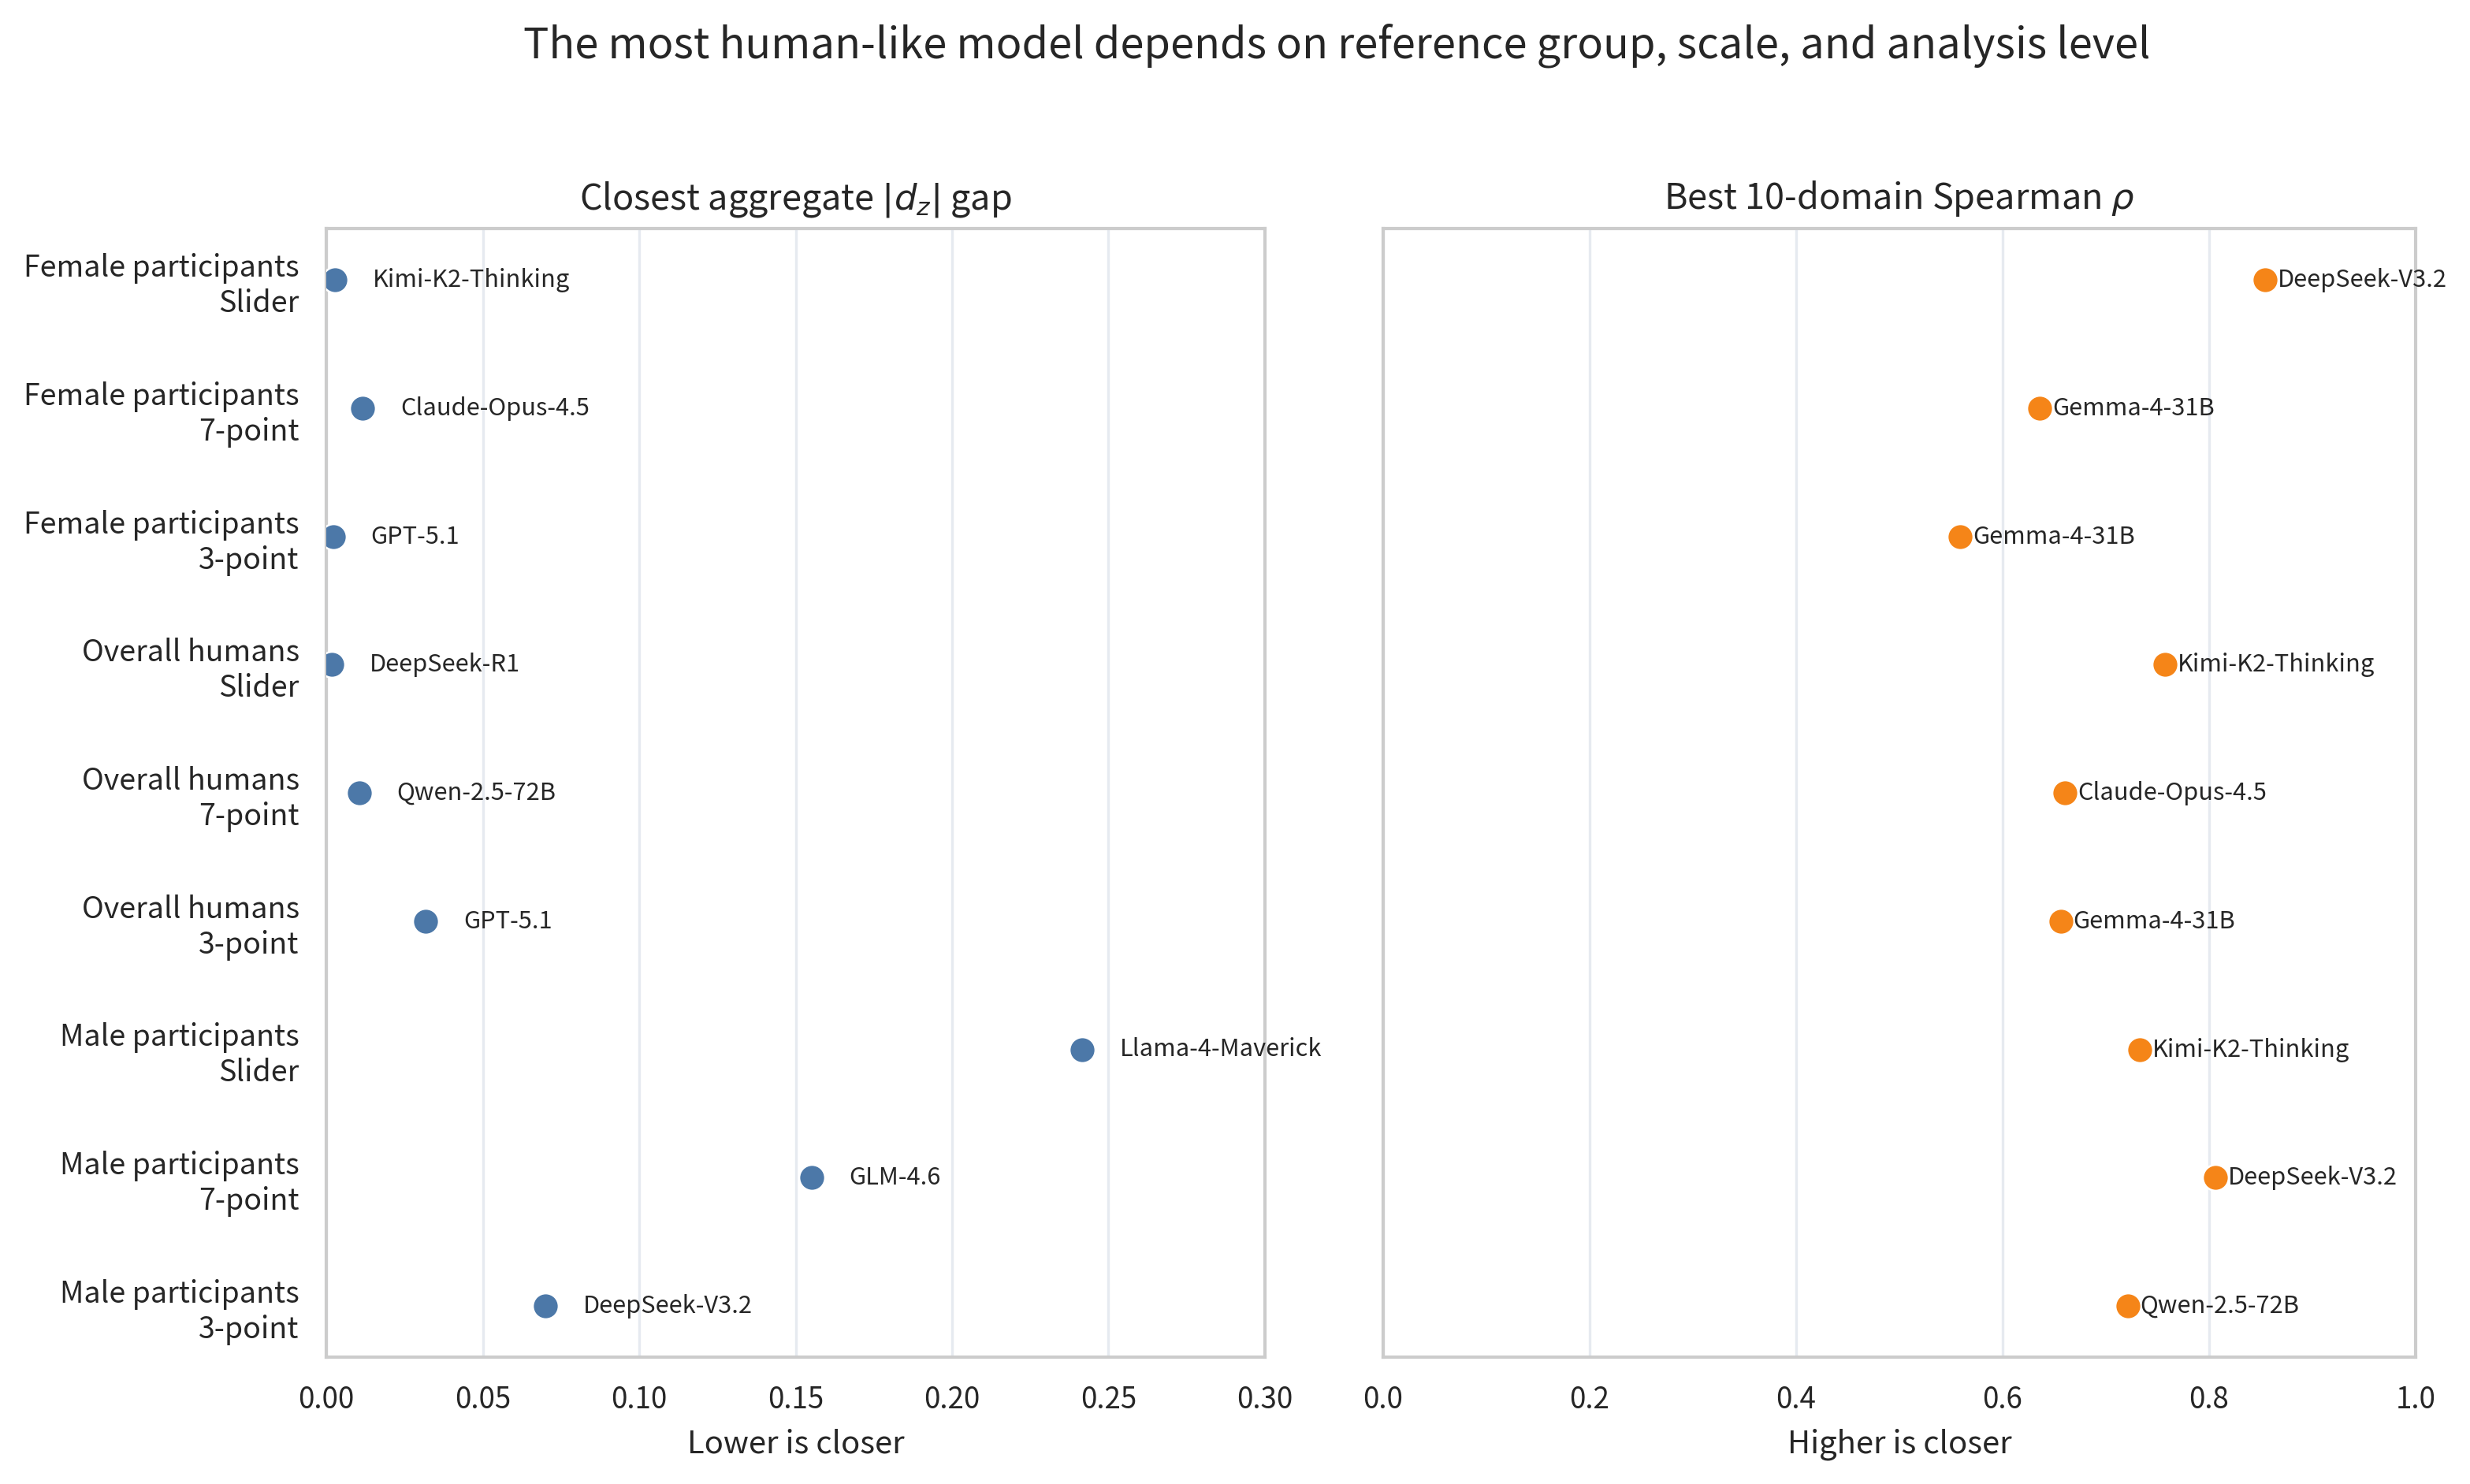
\includegraphics[width=\linewidth]{fig_r6_similarity_by_analysis_level_forest.pdf}
    \caption{Closest LLM by analysis level. No model occupies the closest position on all three panels.}
    \label{fig:levels-forest}
  \end{subfigure}\hfill
  \begin{subfigure}[t]{0.49\linewidth}
    \centering
    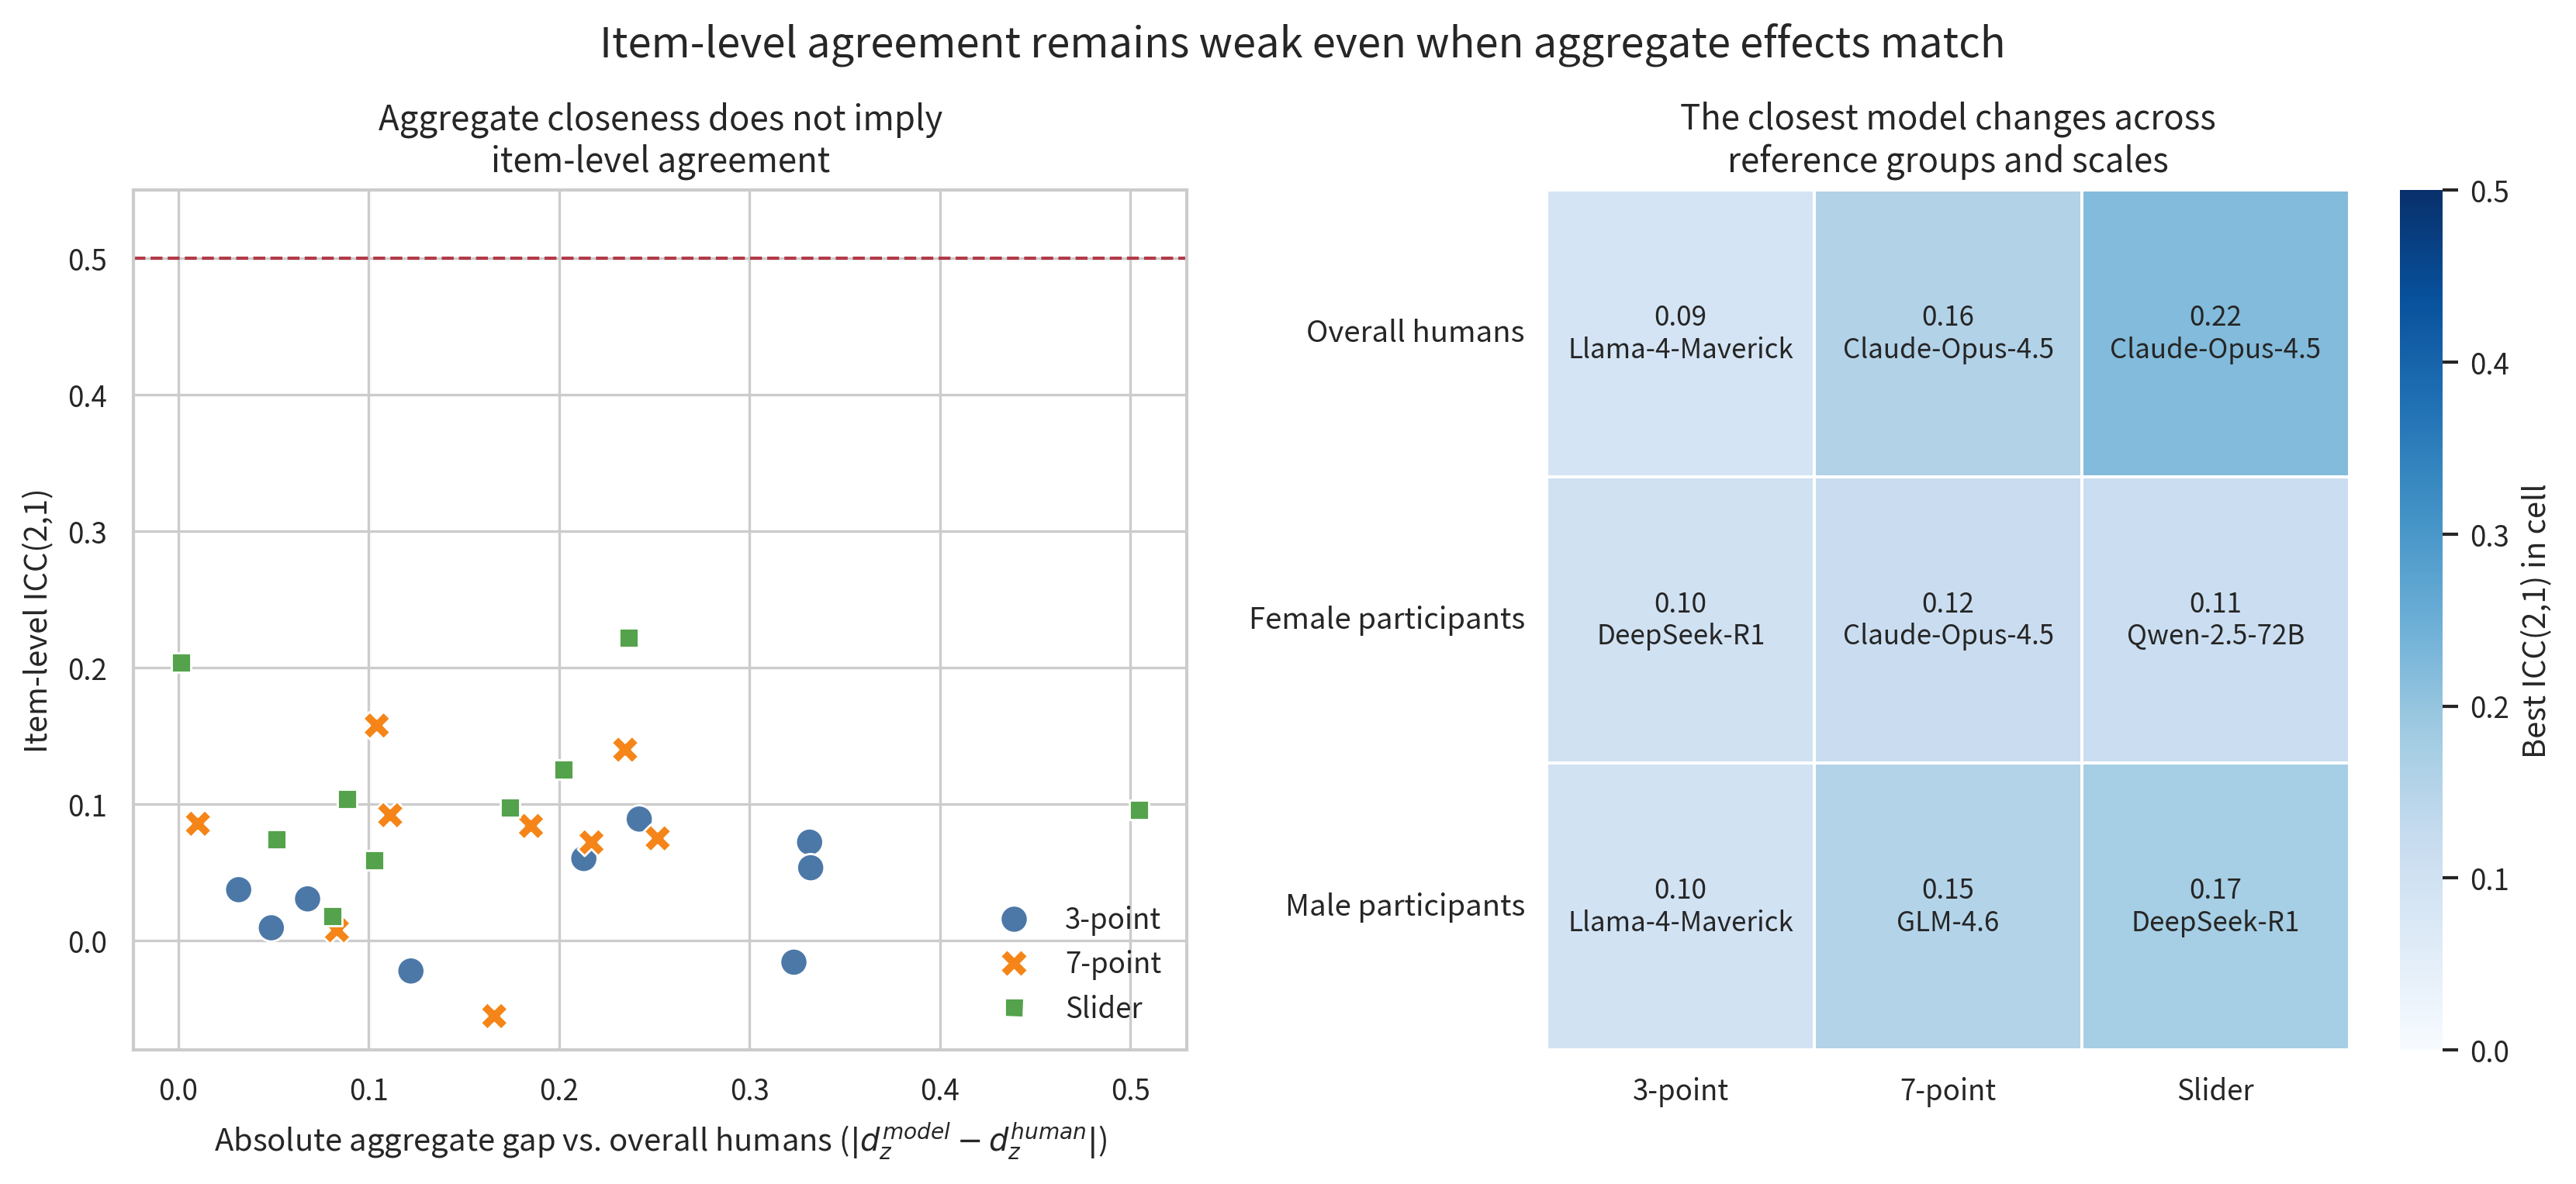
\includegraphics[width=\linewidth]{fig_r6_aggregate_item_dissociation.pdf}
    \caption{Aggregate similarity does not imply item-level similarity. Each point is an LLM; the x-axis is the absolute aggregate $d_z$ gap to a human reference, the y-axis is the item-level ICC(2,1).}
    \label{fig:levels-dissociation}
  \end{subfigure}
  \caption{Human--LLM agreement viewed at three analytic levels.}
  \label{fig:levels}
\end{figure}

\subsection{Theoretical Implications}

Humans and LLMs see the same gender-attacking effect in the same content regions. When the attack content is held fixed and only the target gender changes, both rate the female-targeted version as more attacking on average, and both place the largest gaps in attacks on sexualization and appearance. The domain-profile agreement is partial: seven of the nine best-model Spearman correlations exceeded a permutation-null cutoff of $|\rho|\!\approx\!0.65$ for 10 domains, while two female-anchored cells did not. Beyond this shared structure, the two rater types were not interchangeable. The size of the gender-differential gap depended on which human reference group an LLM was compared to: the LLM panel sat between the male-participant and pooled-human references on the 3-point scale, and shifted toward and above the female-participant reference on the slider. Item-level intraclass correlations remained in the $0.089$--$0.222$ range even when aggregate $d_z$ values nearly coincided, so two raters that agree on the average effect can still disagree about which individual sentences carry it. Agreement is observed at the level of \emph{direction and broad content structure}, while divergence is observed at the level of \emph{magnitude}, \emph{response-scale behaviour}, and \emph{item-level ordering}. Such a pattern fits an account in which LLMs encode gender as a coarse-grained signal of attack severity while diverging from human raters in the finer-grained perceptual structure of individual sentences. Cross-model variability, most clearly Gemma-4-31B rising from $d_z=0.408$ to $1.016$ across formats, is not adjudicated by our design and is consistent with a \emph{sensitivity-calibrated} sub-account, under which safety- or instruction-tuning makes some models more responsive on protected-attribute content as the scale gives them more numerical room to express that response. Plausible moderators of this LLM-to-LLM variability include parameter count, the tuning regime (instruction-tuning vs. safety-oriented RLHF vs. reasoning-oriented RL), and the system-prompt formulation used at inference; separating their contributions requires a controlled comparison that varies each moderator while holding the others fixed, which the present panel of nine production LLMs is too small to support and which we leave to future work.

\subsection{Methodological Implications}

Reporting a single agreement number between an LLM and a pooled human reference under a single response format hides the variation that this study makes visible. The same panel of nine LLMs that looks above the pooled-human $d_z$ on the slider sits below it on the 3-point scale, and the same panel that nearly matches humans in aggregate $d_z$ shows item-level intraclass correlations below $0.25$ (Fig.~\ref{fig:levels}). A pooled-human gold label also hides the subgroup structure of the human side, since female and male participants produced systematically different $\Delta_{F-M}$ values, so an aggregate similarity claim is not interpretable without naming the human reference. Domain-level Spearman correlations need a permutation-null baseline because with only 10 attack domains random ranking already covers a wide $\rho$ band, so a moderate Spearman value is not automatically informative. Controlled minimal-pair stimuli are needed to isolate target gender from content extremity, which is confounded with target identity in naturally occurring corpora, and the agreement construct must be reported as a structured profile across direction, magnitude, domain profile, and item level, against a named human reference group and under a named response format, rather than as a single global agreement number.

\subsection{Practical Implications}

For Chinese social-computing pipelines that use LLM ratings of gendered attack content, three concrete uses are constrained by these findings. First, an LLM rating against a single pooled-human label cannot be interpreted as the LLM's match to female perceivers' judgements even when the aggregate $d_z$ values are close, because pooled-human aggregates are mixtures of subgroups with materially different $\Delta_{F-M}$. Second, an aggregate-level agreement statistic cannot certify item-level interchangeability for moderation pipelines that act on individual posts, since aggregate similarity coexists with $\mathrm{ICC}(2,1) \leq 0.222$ at the item level. Third, a model-versus-human comparison conducted on a coarse 3-point scale does not transfer to deployment settings that elicit finer-grained ratings (such as continuous toxicity scores), because the LLM-to-human gap is not monotone in scale granularity: most LLMs grow as the scale becomes finer while humans flatten or decline. Pipelines that depend on any of these three substitutions need an alignment profile specific to their deployed reference group, scale, and analytic level rather than a transferred single-number agreement claim.

\section{Limitations and Conclusion}

The stimuli are Chinese, and the participant pool is a young online Chinese sample rather than a nationally representative population. The model panel is a November 2025 snapshot; later model versions may differ. The minimal-pair design isolates target gender but does not capture multimodal cues, reply context, or platform-specific pragmatics. Participant gender is treated as binary because the available sample supports only that contrast at stable cell sizes. The two accounts compared here exhaust neither the space of possible LLM-rater models nor the space of cross-model differences within the panel.

Within these limits, the pattern of human--LLM agreement is clear: on the same Chinese gender-reversal minimal pairs, humans and LLMs share the direction of the effect and locate its largest values in attacks on sexualization and appearance, but diverge on its magnitude, on how that magnitude moves with the response format, and on which individual sentences carry it. Social-computing evaluations of LLM ratings of subjective content should therefore be reported as a structured profile across direction, magnitude, domain profile, and item level, against a named human reference group and under a named response format, rather than as a single global agreement score.

\begin{credits}
\subsubsection{\ackname} This study was not supported by external funding.
\subsubsection{\discintname} The authors have no competing interests to declare that are relevant to the content of this article.
\end{credits}

\begin{thebibliography}{20}

\bibitem{jiang2021}
Jiang, A., Yang, X., Liu, Y., Zubiaga, A.: SWSR: A Chinese dataset and lexicon for online sexism detection. Online Social Networks and Media 27, 100182 (2021)

\bibitem{jingschmidt2018}
Jing-Schmidt, Z., Peng, X.: The sluttified sex: Verbal misogyny reflects and reinforces gender order in wireless China. Language in Society 47(3), 385--408 (2018)

\bibitem{liao2024}
Liao, S.: The platformization of misogyny: Popular media, gender politics, and misogyny in China's state-market nexus. Media, Culture \& Society 46(1), 191--207 (2024)

\bibitem{mathew2021}
Mathew, B., Saha, P., Yimam, S.M., Biemann, C., Goyal, P., Mukherjee, A.: HateXplain: A benchmark dataset for explainable hate speech detection. In: AAAI, vol. 35, pp. 14867--14875 (2021)

\bibitem{lozano2008}
Lozano, L.M., Garc\'ia-Cueto, E., Mu\~niz, J.: Effect of the number of response categories on the reliability and validity of rating scales. Methodology 4(2), 73--79 (2008)

\bibitem{preston2000}
Preston, C.C., Colman, A.M.: Optimal number of response categories in rating scales. Acta Psychologica 104(1), 1--15 (2000)

\bibitem{cowan1996}
Cowan, G., Hodge, C.: Judgments of hate speech: The effects of target group, publicness, and behavioral responses of the target. Journal of Applied Social Psychology 26(4), 355--374 (1996)

\bibitem{giorgi2025}
Giorgi, T., Cima, L., Fagni, T., Avvenuti, M., Cresci, S.: Human and LLM biases in hate speech annotations: A socio-demographic analysis of annotators and targets. In: Proceedings of the International AAAI Conference on Web and Social Media (ICWSM), vol. 19 (2025)

\bibitem{sap2019}
Sap, M., Card, D., Gabriel, S., Choi, Y., Smith, N.A.: The risk of racial bias in hate speech detection. In: Proceedings of the 57th Annual Meeting of the Association for Computational Linguistics, pp. 1668--1678 (2019)

\bibitem{larimore2021}
Larimore, S., Kennedy, I., Haskett, B., Arseniev-Koehler, A.: Reconsidering annotator disagreement about racist language: Noise or signal? In: Proceedings of the Ninth International Workshop on Natural Language Processing for Social Media, pp. 81--90 (2021)

\bibitem{santy2023}
Santy, S., Liang, J.T., Le Bras, R., Reinecke, K., Sap, M.: NLPositionality: Characterizing design biases of datasets and models. In: Proceedings of the 61st Annual Meeting of the Association for Computational Linguistics, pp. 9080--9102 (2023)

\bibitem{schoenebeck2023}
Schoenebeck, S., Batool, A., Do, G., Darling, S., Grill, G., Wilkinson, D., Khan, M., Toyama, K., Ashwell, L.: Online harassment in majority contexts: Examining harms and remedies across countries. In: Proceedings of the 2023 CHI Conference on Human Factors in Computing Systems, Article 485 (2023)

\bibitem{davani2022}
Davani, A.M., D\'iaz, M., Prabhakaran, V.: Dealing with disagreements: Looking beyond the majority vote in subjective annotations. Transactions of the Association for Computational Linguistics 10, 92--110 (2022)

\bibitem{orlikowski2025}
Orlikowski, M., Pei, J., R\"ottger, P., Cimiano, P., Jurgens, D., Hovy, D.: Beyond demographics: Fine-tuning large language models to predict individuals' subjective text perceptions. In: Findings of the Association for Computational Linguistics (2025)

\bibitem{sun2025}
Sun, H., Pei, J., Choi, M., Jurgens, D.: Aligning with whom? Large language models have gender and racial biases in subjective NLP tasks. arXiv preprint arXiv:2311.09730 (2025)

\bibitem{he2024}
He, X., Lin, Z., Gong, Y., Jin, A.L., Zhang, H., Lin, C., Jiao, J., Yiu, S.M., Duan, N., Chen, W.: AnnoLLM: Making large language models to be better crowdsourced annotators. In: Proceedings of the 2024 Conference of the North American Chapter of the Association for Computational Linguistics, pp. 165--190 (2024)

\bibitem{ziems2024}
Ziems, C., Held, W., Shaikh, O., Chen, J., Zhang, Z., Yang, D.: Can large language models transform computational social science? Computational Linguistics 50(1), 237--291 (2024)

\bibitem{chiu2022}
Chiu, K.-L., Collins, A., Alexander, R.: Detecting hate speech with GPT-3. arXiv preprint arXiv:2103.12407 (2022)

\bibitem{davidson2026}
Davidson, T.: Multimodal large language models can make context-sensitive hate speech evaluations aligned with human judgement. Nature Human Behaviour 10, 514--530 (2026)

\bibitem{ribeiro2020}
Ribeiro, M.T., Wu, T., Guestrin, C., Singh, S.: Beyond accuracy: Behavioral testing of NLP models with CheckList. In: Proceedings of the 58th Annual Meeting of the Association for Computational Linguistics, pp. 4902--4912 (2020)

\bibitem{rottger2021}
R\"ottger, P., Vidgen, B., Nguyen, D., Waseem, Z., Margetts, H., Pierrehumbert, J.B.: HateCheck: Functional tests for hate speech detection models. In: Proceedings of the 59th Annual Meeting of the Association for Computational Linguistics, pp. 41--58 (2021)

\end{thebibliography}

\end{document}
